%MDA diagram
\begin{figure}[ht]
\centering

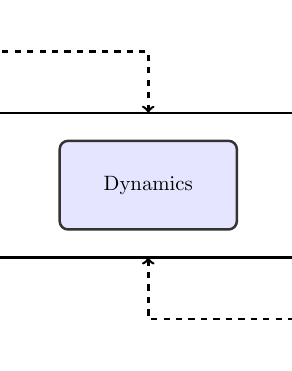
\begin{tikzpicture}[squarednode/.style={rectangle, 
					rounded corners, 
					very thick,
 					minimum width=3cm,
					minimum height=1.5cm,
					draw=black!80, 
					fill=green!10},
					squarednode2/.style={rectangle, 
					rounded corners, 
					very thick,
 					minimum width=3cm,
					minimum height=1.5cm,
					draw=black!80, 
					fill=blue!10},
					squarednode3/.style={rectangle, 
					rounded corners, 
					very thick,
 					minimum width=3cm,
					minimum height=1.5cm,
					draw=black!80, 
					fill=red!10}
					]
					
% To reduce all image, transform canvas
% forgets about image size, so 
% we need a bounding box
% This is lame, but works with Eduardo Thesis´s image (now black and white for elegance)

% don´t ask me about theses limits
% I just tried until I found which ones
%workded
\useasboundingbox (3,-2) rectangle (6,2);
\scope[transform canvas={scale=.75}]
         % Your actual drawing


%MDA nodes
\node[squarednode]  (m) [anchor = west]{Mechanics};
\node[squarednode2]  (d) [right of = m, node distance=3cm, anchor=west] {Dynamics};
\node[squarednode3]  (a) [right of = d, node distance=3cm, anchor=west] {Aesthetics};

%paths designer
%\path [-latex,  black, very thick] ([yshift=1ex]m.east) edge coordinate[midway](designerPath1) ([yshift=1ex]d.west);
%\path [-latex,  black, very thick] ([yshift=1ex]d.east) edge coordinate[midway](designerPath2) ([yshift=1ex]a.west);

% new designer path
\path[-latex, black, very thick] ([yshift=-3ex]a.south) edge  coordinate[midway](playerPathnew) ([yshift=-3ex]m.south);

%paths player
%\path [latex-, black, very thick] ([yshift=-1ex]m.east) edge  coordinate[midway](playerPath1)([yshift=-1ex]d.west);
%\path [latex-, black, very thick] ([yshift=-1ex]d.east) edge coordinate[midway](playerPath2) ([yshift=-1ex]a.west);

%new player path
\path[-latex, black, very thick] ([yshift=3ex]m.north) edge  coordinate[midway](designerPathnew) ([yshift=3ex]a.north);

%designer legend
\node [draw] (designerLegend) [above of = m, align=center, node distance=2cm, anchor=south]{\small Designer's Perspective};
\draw [dashed,<-,very thick](designerPathnew.north) |- (designerLegend.east);
%\draw [dashed,<-,very thick](designerPath2.north) |- (designerLegend.east);
%\draw [dashed,<-](designerPath2.north) |- (designerLegend.east);

%player legend
\node [draw] (playerLegend) [below of = a, align=center, node distance=2cm, anchor=north]{\small Player's Perspective};
%\draw[dashed, <-](playerPath1.south) |- (playerLegend.west);
\draw[dashed, <-,very thick](playerPathnew.south) |- (playerLegend.west);
%\draw[dashed, <-,very thick](playerPath1.south) |- (playerLegend.west);
    \endscope
\end{tikzpicture}
\caption{MDA diagram}
\label{fig:MDA_diagram}
\end{figure}